\iffalse
\documentclass[journal,12pt,two column]{IEEEtran}
%\usepackage{setspace}
\usepackage{listings}
\usepackage{amssymb}
\usepackage[cmex10]{amsmath}
\usepackage{amsthm}
\usepackage[export]{adjustbox}
\usepackage{bm}
\def\inputGnumericTable{} 

\usepackage[latin1]{inputenc}                                 
\usepackage{color}                                            
\usepackage{array} 
\usepackage{longtable} 
\usepackage{calc}                                             
\usepackage{multirow}                                         
\usepackage{hhline}                                           
\usepackage{ifthen}  
\usepackage{mathtools}
\usepackage{tikz}
\usepackage{listings}
\usepackage{color}                                            %%
\usepackage{array}                                            %%
\usepackage{caption} 
\usepackage{graphicx}

\title{A1110 Assignment 3 \\ 12.13.1.15}
\author{K.SaiTeja \\ AI22BTECH11014}
\providecommand{\pr}[1]{\ensuremath{\Pr\left(#1\right)}}
\providecommand{\qfunc}[1]{\ensuremath{Q\left(#1\right)}}
\providecommand{\sbrak}[1]{\ensuremath{{}\left[#1\right]}}
\providecommand{\lsbrak}[1]{\ensuremath{{}\left[#1\right.}}
\providecommand{\rsbrak}[1]{\ensuremath{{}\left.#1\right]}}
\providecommand{\brak}[1]{\ensuremath{\left(#1\right)}}
\providecommand{\lbrak}[1]{\ensuremath{\left(#1\right.}}
\providecommand{\rbrak}[1]{\ensuremath{\left.#1\right)}}
\providecommand{\cbrak}[1]{\ensuremath{\left\{#1\right\}}}
\providecommand{\lcbrak}[1]{\ensuremath{\left\{#1\right.}}
\providecommand{\rcbrak}[1]{\ensuremath{\left.#1\right\}}}
\newcommand*{\permcomb}[4][0mu]{{{}^{#3}\mkern#1#2_{#4}}}
\newcommand*{\perm}[1][-3mu]{\permcomb[#1]{P}}
\newcommand*{\comb}[1][-1mu]{\permcomb[#1]{C}}

\renewcommand{\thetable}{\arabic{table}} 
\newcommand{\question}{\noindent \textbf{Question: }}	
\newcommand{\solution}{\noindent \textbf{Solution: }}
\providecommand{\mbf}{\mathbf}
\providecommand{\pr}[1]{\ensuremath{\Pr\left(#1\right)}}
\providecommand{\prt}[2]{\ensuremath{P_{#1}^{\left(#2\right)} }}        % own macro for this question
\providecommand{\qfunc}[1]{\ensuremath{Q\left(#1\right)}}
\providecommand{\sbrak}[1]{\ensuremath{{}\left[#1\right]}}      % []
\providecommand{\lsbrak}[1]{\ensuremath{{}\left[#1\right.}}
\providecommand{\rsbrak}[1]{\ensuremath{{}\left.#1\right]}}
\providecommand{\brak}[1]{\ensuremath{\left(#1\right)}}         % ()
\providecommand{\lbrak}[1]{\ensuremath{\left(#1\right.}}
\providecommand{\rbrak}[1]{\ensuremath{\left.#1\right)}}
\providecommand{\cbrak}[1]{\ensuremath{\left\{#1\right\}}}      % {}
\providecommand{\lcbrak}[1]{\ensuremath{\left\{#1\right.}}
\providecommand{\rcbrak}[1]{\ensuremath{\left.#1\right\}}}
\theoremstyle{remark}
\newtheorem{rem}{Remark}
\newcommand{\sgn}{\mathop{\mathrm{sgn}}}
\providecommand{\abs}[1]{\ensuremath{\left\vert#1\right\vert}}
\providecommand{\res}[1]{\Res\displaylimits_{#1}} 
\providecommand{\norm}[1]{\ensuremath{\left\lVert#1\right\rVert}}
%\providecommand{\norm}[1]{\lVert#1\rVert}
\providecommand{\mtx}[1]{\mathbf{#1}}
\providecommand{\mean}[1]{\ensuremath{E\left[ #1 \right]}}
\providecommand{\fourier}{\overset{\mathcal{F}}{ \rightleftharpoons}}
%\providecommand{\hilbert}{\overset{\mathcal{H}}{ \rightleftharpoons}}
\providecommand{\system}{\overset{\mathcal{H}}{ \longleftrightarrow}}
	%\newcommand{\solution}[2]{\textbf{Solution:}{#1}}
\newcommand{\cosec}{\,\text{cosec}\,}
\providecommand{\dec}[2]{\ensuremath{\overset{#1}{\underset{#2}{\gtrless}}}}
\newcommand{\myvec}[1]{\ensuremath{\begin{pmatrix}#1\end{pmatrix}}}
\newcommand{\mydet}[1]{\ensuremath{\begin{vmatrix}#1\end{vmatrix}}}
%
%not used because document is short:
%\numberwithin{equation}{section}
%\numberwithin{figure}{section}
%\numberwithin{table}{section}
%\numberwithin{equation}{section}
%\numberwithin{problem}{section}
%\numberwithin{definition}{section}
\makeatletter
\@addtoreset{figure}{problem}
\makeatother

\let\StandardTheFigure\thefigure
\let\vec\mathbf
%\renewcommand{\thefigure}{\theproblem.\arabic{figure}}
    %\renewcommand{\thefigure}{\theproblem}
%\setlist[enumerate,1]{before=\renewcommand\theequation{\theenumi.\arabic{equation}}
%\counterwithin{equation}{enumi}
%\renewcommand{\theequation}{\arabic{subsection}.\arabic{equation}}

\def\putbox#1#2#3{\makebox[0in][l]{\makebox[#1][l]{}\raisebox{\baselineskip}[0in][0in]{\raisebox{#2}[0in][0in]{#3}}}}
     \def\rightbox#1{\makebox[0in][r]{#1}}
     \def\centbox#1{\makebox[0in]{#1}}
     \def\topbox#1{\raisebox{-\baselineskip}[0in][0in]{#1}}
     \def\midbox#1{\raisebox{-0.5\baselineskip}[0in][0in]{#1}}
\vspace{3cm}

%\renewcommand{\thefigure}{\theenumi}
%\renewcommand{\thetable}{\theenumi}
%\renewcommand{\theequation}{\theenumi}

\begin{document}
\maketitle
\question
\solution\tableofcontents
\fi
\begin{enumerate}
	\item  See 
        \tabref{tab:ncert/12/13/1/15m/States}	
	and 
        \figref{fig:ncert/12/13/1/15m/ markov_chain}.
    \begin{table}[ht!]
        \centering
    	%%%%%%%%%%%%%%%%%%%%%%%%%%%%%%%%%%%%%%%%%%%%%%%%%%%%%%%%%%%%%%%%%%%%%%
%%                                                                  %%
%%  This is the header of a LaTeX2e file exported from Gnumeric.    %%
%%                                                                  %%
%%  This file can be compiled as it stands or included in another   %%
%%  LaTeX document. The table is based on the longtable package so  %%
%%  the longtable options (headers, footers...) can be set in the   %%
%%  preamble section below (see PRAMBLE).                           %%
%%                                                                  %%
%%  To include the file in another, the following two lines must be %%
%%  in the including file:                                          %%
%%        \def\inputGnumericTable{}                                 %%
%%  at the beginning of the file and:                               %%
%%        \input{name-of-this-file.tex}                             %%
%%  where the table is to be placed. Note also that the including   %%
%%  file must use the following packages for the table to be        %%
%%  rendered correctly:                                             %%
%%    \usepackage[latin1]{inputenc}                                 %%
%%    \usepackage{color}                                            %%
%%    \usepackage{array}                                            %%
%%    \usepackage{longtable}                                        %%
%%    \usepackage{calc}                                             %%
%%    \usepackage{multirow}                                         %%
%%    \usepackage{hhline}                                           %%
%%    \usepackage{ifthen}                                           %%
%%  optionally (for landscape tables embedded in another document): %%
%%    \usepackage{lscape}                                           %%
%%                                                                  %%
%%%%%%%%%%%%%%%%%%%%%%%%%%%%%%%%%%%%%%%%%%%%%%%%%%%%%%%%%%%%%%%%%%%%%%



%%  This section checks if we are begin input into another file or  %%
%%  the file will be compiled alone. First use a macro taken from   %%
%%  the TeXbook ex 7.7 (suggestion of Han-Wen Nienhuys).            %%
\def\ifundefined#1{\expandafter\ifx\csname#1\endcsname\relax}


%%  Check for the \def token for inputed files. If it is not        %%
%%  defined, the file will be processed as a standalone and the     %%
%%  preamble will be used.                                          %%
\ifundefined{inputGnumericTable}

%%  We must be able to close or not the document at the end.        %%
	\def\gnumericTableEnd{\end{document}}


%%%%%%%%%%%%%%%%%%%%%%%%%%%%%%%%%%%%%%%%%%%%%%%%%%%%%%%%%%%%%%%%%%%%%%
%%                                                                  %%
%%  This is the PREAMBLE. Change these values to get the right      %%
%%  paper size and other niceties.                                  %%
%%                                                                  %%
%%%%%%%%%%%%%%%%%%%%%%%%%%%%%%%%%%%%%%%%%%%%%%%%%%%%%%%%%%%%%%%%%%%%%%

	\documentclass[12pt%
			  %,landscape%
                    ]{report}
       \usepackage[latin1]{inputenc}
       \usepackage{fullpage}
       \usepackage{color}
       \usepackage{array}
       \usepackage{longtable}
       \usepackage{calc}
       \usepackage{multirow}
       \usepackage{hhline}
       \usepackage{ifthen}

	\begin{document}


%%  End of the preamble for the standalone. The next section is for %%
%%  documents which are included into other LaTeX2e files.          %%
\else

%%  We are not a stand alone document. For a regular table, we will %%
%%  have no preamble and only define the closing to mean nothing.   %%
    \def\gnumericTableEnd{}

%%  If we want landscape mode in an embedded document, comment out  %%
%%  the line above and uncomment the two below. The table will      %%
%%  begin on a new page and run in landscape mode.                  %%
%       \def\gnumericTableEnd{\end{landscape}}
%       \begin{landscape}


%%  End of the else clause for this file being \input.              %%
\fi

%%%%%%%%%%%%%%%%%%%%%%%%%%%%%%%%%%%%%%%%%%%%%%%%%%%%%%%%%%%%%%%%%%%%%%
%%                                                                  %%
%%  The rest is the gnumeric table, except for the closing          %%
%%  statement. Changes below will alter the table's appearance.     %%
%%                                                                  %%
%%%%%%%%%%%%%%%%%%%%%%%%%%%%%%%%%%%%%%%%%%%%%%%%%%%%%%%%%%%%%%%%%%%%%%

\providecommand{\gnumericmathit}[1]{#1} 
%%  Uncomment the next line if you would like your numbers to be in %%
%%  italics if they are italizised in the gnumeric table.           %%
%\renewcommand{\gnumericmathit}[1]{\mathit{#1}}
\providecommand{\gnumericPB}[1]%
{\let\gnumericTemp=\\#1\let\\=\gnumericTemp\hspace{0pt}}
 \ifundefined{gnumericTableWidthDefined}
        \newlength{\gnumericTableWidth}
        \newlength{\gnumericTableWidthComplete}
        \newlength{\gnumericMultiRowLength}
        \global\def\gnumericTableWidthDefined{}
 \fi
%% The following setting protects this code from babel shorthands.  %%
 \ifthenelse{\isundefined{\languageshorthands}}{}{\languageshorthands{english}}
%%  The default table format retains the relative column widths of  %%
%%  gnumeric. They can easily be changed to c, r or l. In that case %%
%%  you may want to comment out the next line and uncomment the one %%
%%  thereafter                                                      %%
\providecommand\gnumbox{\makebox[0pt]}
%%\providecommand\gnumbox[1][]{\makebox}

%% to adjust positions in multirow situations                       %%
\setlength{\bigstrutjot}{\jot}
\setlength{\extrarowheight}{\doublerulesep}

%%  The \setlongtables command keeps column widths the same across  %%
%%  pages. Simply comment out next line for varying column widths.  %%
\setlongtables

\setlength\gnumericTableWidth{%
	38pt+%
	155pt+%
0pt}
\def\gumericNumCols{2}
\setlength\gnumericTableWidthComplete{\gnumericTableWidth+%
         \tabcolsep*\gumericNumCols*2+\arrayrulewidth*\gumericNumCols}
\ifthenelse{\lengthtest{\gnumericTableWidthComplete > \linewidth}}%
         {\def\gnumericScale{1*\ratio{\linewidth-%
                        \tabcolsep*\gumericNumCols*2-%
                        \arrayrulewidth*\gumericNumCols}%
{\gnumericTableWidth}}}%
{\def\gnumericScale{1}}

%%%%%%%%%%%%%%%%%%%%%%%%%%%%%%%%%%%%%%%%%%%%%%%%%%%%%%%%%%%%%%%%%%%%%%
%%                                                                  %%
%% The following are the widths of the various columns. We are      %%
%% defining them here because then they are easier to change.       %%
%% Depending on the cell formats we may use them more than once.    %%
%%                                                                  %%
%%%%%%%%%%%%%%%%%%%%%%%%%%%%%%%%%%%%%%%%%%%%%%%%%%%%%%%%%%%%%%%%%%%%%%

\ifthenelse{\isundefined{\gnumericColA}}{\newlength{\gnumericColA}}{}\settowidth{\gnumericColA}{\begin{tabular}{@{}p{38pt*\gnumericScale}@{}}x\end{tabular}}
\ifthenelse{\isundefined{\gnumericColB}}{\newlength{\gnumericColB}}{}\settowidth{\gnumericColB}{\begin{tabular}{@{}p{155pt*\gnumericScale}@{}}x\end{tabular}}

\begin{tabular}[c]{%
	b{\gnumericColA}%
	b{\gnumericColB}%
	}

%%%%%%%%%%%%%%%%%%%%%%%%%%%%%%%%%%%%%%%%%%%%%%%%%%%%%%%%%%%%%%%%%%%%%%
%%  The longtable options. (Caption, headers... see Goosens, p.124) %%
%	\caption{The Table Caption.}             \\	%
% \hline	% Across the top of the table.
%%  The rest of these options are table rows which are placed on    %%
%%  the first, last or every page. Use \multicolumn if you want.    %%

%%  Header for the first page.                                      %%
%	\multicolumn{2}{c}{The First Header} \\ \hline 
%	\multicolumn{1}{c}{colTag}	%Column 1
%	&\multicolumn{1}{c}{colTag}	\\ \hline %Last column
%	\endfirsthead

%%  The running header definition.                                  %%
%	\hline
%	\multicolumn{2}{l}{\ldots\small\slshape continued} \\ \hline
%	\multicolumn{1}{c}{colTag}	%Column 1
%	&\multicolumn{1}{c}{colTag}	\\ \hline %Last column
%	\endhead

%%  The running footer definition.                                  %%
%	\hline
%	\multicolumn{2}{r}{\small\slshape continued\ldots} \\
%	\endfoot

%%  The ending footer definition.                                   %%
%	\multicolumn{2}{c}{That's all folks} \\ \hline 
%	\endlastfoot
%%%%%%%%%%%%%%%%%%%%%%%%%%%%%%%%%%%%%%%%%%%%%%%%%%%%%%%%%%%%%%%%%%%%%%

\hhline{|-|-}
	 \multicolumn{1}{|p{\gnumericColA}|}%
	{\gnumericPB{\centering}\gnumbox{\textbf{i}}}
	&\multicolumn{1}{p{\gnumericColB}|}%
	{\gnumericPB{\centering}\gnumbox{\textbf{State $\brak{e_i}$} }}
\\
\hhline{|--|}
	 \multicolumn{1}{|p{\gnumericColA}|}%
	{\gnumericPB{\centering}\gnumbox{0}}
	&\multicolumn{1}{p{\gnumericColB}|}%
	{\gnumericPB{\centering}\gnumbox{$Y=3$ OR $Y=6$}}
\\
\hhline{|--|}
	 \multicolumn{1}{|p{\gnumericColA}|}%
	{\gnumericPB{\centering}\gnumbox{1}}
	&\multicolumn{1}{p{\gnumericColB}|}%
	{\gnumericPB{\centering}\gnumbox{$\sum \brak{Y= k}; k \in \cbrak{1,2,4,5} $ }}
\\
\hhline{|--|}
	 \multicolumn{1}{|p{\gnumericColA}|}%
	{\gnumericPB{\centering}\gnumbox{2}}
	&\multicolumn{1}{p{\gnumericColB}|}%
	{\gnumericPB{\centering}\gnumbox{Obtaining heads from coin toss }}
\\
\hhline{|--|}
	 \multicolumn{1}{|p{\gnumericColA}|}%
	{\gnumericPB{\centering}\gnumbox{3}}
	&\multicolumn{1}{p{\gnumericColB}|}%
	{\gnumericPB{\centering}\gnumbox{Obtaining tails from coin toss}}
\\
\hhline{|-|-|}
\end{tabular}
\ifthenelse{\isundefined{\languageshorthands}}{}{\languageshorthands{\languagename}}
\gnumericTableEnd



        \caption{States in Markov Chain}
        \label{tab:ncert/12/13/1/15m/States}	
    \end{table}
\begin{figure}[!ht]
        \centering
        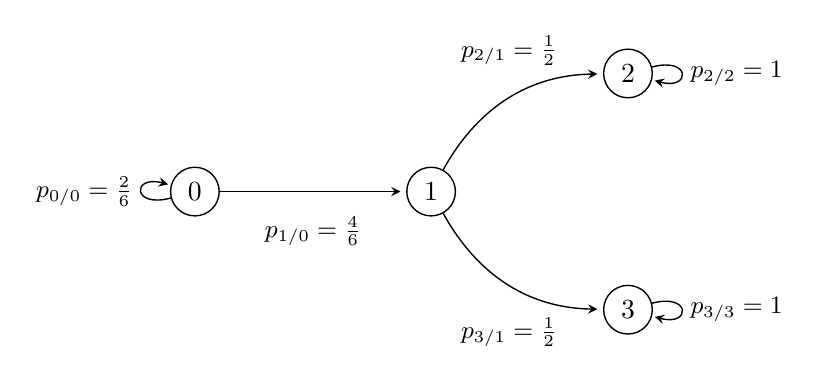
\begin{tikzpicture}[->, >= stealth, shorten >=2pt , line width =0.5 pt, node distance =2 cm]//
\node [circle, draw] (0) at (0, 1.5) {$0$};
  \node [circle, draw] (1) at (3, 1.5) {$1$};
  \node [circle, draw] (2) at (5.5, 3) {$2$};
  \node [circle, draw] (3) at (5.5, 0) {$3$};
  
  \begin{small}
    \path (0) edge [loop left] node [left] {$p_{0/0} = \frac{2}{6}$} (0);
    \path (0) edge node [below = 0.2cm] {$p_{1/0} = \frac{4}{6}$} (1);
  
    \path (1) edge [bend left] node [above = 0.3cm] {$p_{2/1} = \frac{1}{2}$} (2);
    \path (1) edge [bend right] node [below = 0.3cm] {$p_{3/1} = \frac{1}{2}$} (3);
  
    \path (2) edge [loop right] node {$p_{2/2} = 1$} (2);
    \path (3) edge [loop right] node {$p_{3/3} = 1$} (3);
  \end{small}
        \end{tikzpicture}
  
        \caption{Graph of Markov Chain}
        \label{fig:ncert/12/13/1/15m/ markov_chain}
\end{figure}
\item 
    The state vector is,   
    \begin{align}
        \vec{Q}_n &= \myvec{\prt{0}{n}\\ 
        			        \prt{1}{n} \\
        			        \prt{2}{n} \\
        			        \prt{3}{n} 
        			        }        
    \end{align}    
    The probabilities after one step in time are
    \begin{align}
       \prt{0}{n+1} &= \frac{2}{6} \times \prt{0}{n}  \\
       \prt{1}{n+1} &= \frac{4}{6} \times \prt{0}{n}  \\
       \prt{2}{n+1} &= \frac{1}{2} \times \prt{1}{n} + 1 \times \prt{2}{n}
\\
       \prt{3}{n+1} &= \frac{1}{2} \times \prt{1}{n} + 1 \times \prt{3}{n} 
    \end{align}
   \item  
    The previous equations can be summarized as
    \begin{align}
        \vec{Q}_{n+1} &= \vec{P}\vec{Q}_n 
        \label{eq:ncert/12/13/1/15m/transtition}        
    \end{align}
		Where $\vec{P}$ is the transition probability matrix. Its elements are values of $p_{i|j}$
    \begin{align}
        \vec{P}= \myvec{%%%%%%%%%%%%%%%%%%%%%%%%%%%%%%%%%%%%%%%%%%%%%%%%%%%%%%%%%%%%%%%%%%%%%%
%%                                                                  %%
%%  This is a LaTeX2e table fragment exported from Gnumeric.        %%
%%                                                                  %%
%%%%%%%%%%%%%%%%%%%%%%%%%%%%%%%%%%%%%%%%%%%%%%%%%%%%%%%%%%%%%%%%%%%%%%
\begin{tabular}{|l|l|}\hline
	Pr(Event)	&Value \\ \hline
	Pr($Y$=1 $\mid$ $X$=0) &0.25 \\ \hline
	Pr($Y$=1 $\mid$ $X$=1) &1  \\ \hline
	Pr($X$=0) &0.25 \\ \hline
	Pr($X$=1)	&0.75 \\ \hline
	
\end{tabular}
} 
    \end{align}
\item 
     The given condition is that \lq3 occurs at least once\rq. Let the first occurrence of 3 be the initial state $ \vec{Q}_0$.
    \begin{align}
        \vec{Q}_0 &= \myvec{ 1 \\ 0 \\ 0 \\ 0 } 
    \end{align}
    Using \eqref{eq:ncert/12/13/1/15m/transtition}, further states can be generated.
    \begin{align}
        \vec{Q}_1 &= \vec{P} \vec{Q}_0
            = \myvec{\frac{2}{6} \\[4pt] \frac{4}{6}  \\[4pt] 0 \\ 0}\\
        \vec{Q}_2 &= \vec{P} \vec{Q}_1 = \vec{P}^{2} \vec{Q}_0 
            = \myvec{\frac{4}{9}  \\[4pt] \frac{8}{9}  \\[4pt] \frac{5}{24}\\[4pt] \frac{5}{12}} \\   
        \vdots \\
        \vec{Q}_n &= \vec{P}^{n} \vec{Q}_0
    \end{align}
    \item 
 Now to find the eigen values, 
 \begin{align}
\mydet{\vec{P}-\lambda \vec{I}} &= 0  
\\
 \implies \myvec{%%%%%%%%%%%%%%%%%%%%%%%%%%%%%%%%%%%%%%%%%%%%%%%%%%%%%%%%%%%%%%%%%%%%%%
%%                                                                  %%
%%  This is a LaTeX2e table fragment exported from Gnumeric.        %%
%%                                                                  %%
%%%%%%%%%%%%%%%%%%%%%%%%%%%%%%%%%%%%%%%%%%%%%%%%%%%%%%%%%%%%%%%%%%%%%%

\begin{center}
    \begin{tabular}{|c|c|}
    \hline
	    \textbf{Digit}& \textbf{Favourable} \\ \hline
	    $X_{1}$ 		   & 	$5,7$	\\ \hline
	    $X_{2},X_{3},X_{4}$ 		   & 	$0,1,3,5,7$ \\ \hline

    \end{tabular}
    \end{center}
} &= 0
 \\
	 \implies \lambda\brak{\frac{2}{6} - \lambda}\brak{1 - \lambda^2} &= 0
	 \\
	 \text{or, }\lambda &= \frac{2}{6}, 0 , 1 , 1 
 \end{align}
 The corresponding eigenvectors are
\begin{enumerate}
\item $\lambda = \frac{2}{6}$
\begin{align}
\vec{X} &= \myvec{\frac{-2}{3}\\[4pt] \frac{-4}{3}\\[4pt] 1\\[4pt] 1}
\end{align}
\item $\lambda = 0$
\begin{align}
\vec{X} &= \myvec{0 \\[2pt] -2\\[2pt] 1\\ 1}
\end{align}
\item $\lambda = 1$
\begin{align}
\vec{X} &= \myvec{0 \\ 0 \\ 1 \\ 0},\, 
\myvec{0 \\ 0 \\ 0 \\ 1}\\
\end{align}
\end{enumerate}
resulting in the 
eigenvector matrix
\begin{align}
\vec{S} &= \myvec{\input{ncert/12/13/1/15m/tables/table5.txt}}
\end{align}
Thus, 
\begin{align}
	\vec{P} &= \vec{S}\vec{D}\vec{S}^{-1}
\end{align}
Where $\vec{D}$ is eigenvalue matrix
\begin{align}
\vec{D} &= \myvec{\input{ncert/12/13/1/15m/tables/table6.txt}}
\end{align}
\item
\begin{align}
\vec{P}^{n} &= (\vec{S}\vec{D}\vec{S}^{-1})(\vec{S}\vec{D}\vec{S}^{-1}) \dots (\vec{S}\vec{D}\vec{S}^{-1})\\
\implies  &= \vec{S}\vec{D}^{n}\vec{S}^{-1}\\
\implies \lim_{n \to \infty}\vec{P}^{n} &= \lim_{n \to \infty}\vec{S}\vec{D}^{n}\vec{S}^{-1}
\end{align}
	From 
        \eqref{eq:ncert/12/13/1/15m/transtition},
\begin{align}
\vec{Q}_{n} &= \vec{P}^{n}\vec{Q}_{0}
\end{align}
and
Now,
\begin{align}
\vec{\lim_{n \to \infty}\vec{D}^{n}} &= \myvec{\input{ncert/12/13/1/15m/tables/table7.txt}}\\ 
\implies \vec{\lim_{n \to \infty}\vec{S}\vec{D}^{n}\vec{S}^{-1}} &= \myvec{\input{ncert/12/13/1/15m/tables/table7.txt}} = \vec{\vec{P}^{n}}\\
\implies \vec{Q}_n &= \myvec{\input{ncert/12/13/1/15m/tables/table7.txt}}\vec{Q}_0\\
\implies \vec{Q}_n &= \myvec{0 \\ 0 \\ 0 \\ 0} 
\end{align}
\item 
    Probability of the coin showing tails, given that at least one die shows a 3,
    \begin{align}
       \lim_{n \to \infty} \prt{3}{n} = 0
    \end{align}
   \end{enumerate} 
